\newproblem{07.5a}
{
	Solve and graph on the number line. $$\frac{1}{2}x+3 \leq \frac{3}{4}x$$\begin{onlyproblem}\begin{center}
\includegraphics{numberLineNoNumbersNoTicks}\end{center}\end{onlyproblem} \begin{onlysolution}\begin{center}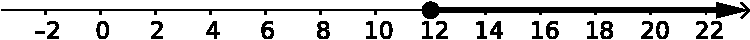
\includegraphics{fig095-07-5-a-answer}\end{center}\end{onlysolution}
}
{
	\begin{tabular}{l r}
	$\dfrac{4}{1}\left(\dfrac{1}{2}x+3\right) \leq \dfrac{4}{1}\left(\dfrac{3}{4}x\right)$ & 1 pt to here \\
	$2x+12\leq 3x$ & 2 pts to here \\
	$12\leq x$ OR $x\geq 12$ & 3 pts to here \\
	 & add 2 pts for correct number line.
	\end{tabular}
}

\newproblem{07.5b}
{
	Solve and graph on the number line. $$\frac{7}{6}x-3 \geq \frac{2}{3}x$$\begin{onlyproblem}\begin{center}
\includegraphics{numberLineNoNumbersNoTicks}\end{center}\end{onlyproblem} \begin{onlysolution}\begin{center}
\includegraphics{fig095-07-5-b-answer}\end{center}\end{onlysolution}
}
{
	\begin{tabular}{l r}
	$\dfrac{6}{1}\left(\dfrac{7}{6}x-3\right) \geq \dfrac{6}{1}\left(\dfrac{2}{3}x\right)$ & 1 pt to here \\
	$7x-18\geq 4x$ & 2 pts to here \\
	$x\geq 6$ OR $6\leq x$ & 3 pts to here \\
	 & add 2 pts for correct number line.
	\end{tabular}
}

\newproblem{07.5c}
{
	Solve and graph on the number line. $$\frac{4}{5}x+2 \leq \frac{3}{10}x$$\begin{onlyproblem}\begin{center}
\includegraphics{numberLineNoNumbersNoTicks}\end{center}\end{onlyproblem} \begin{onlysolution}\begin{center}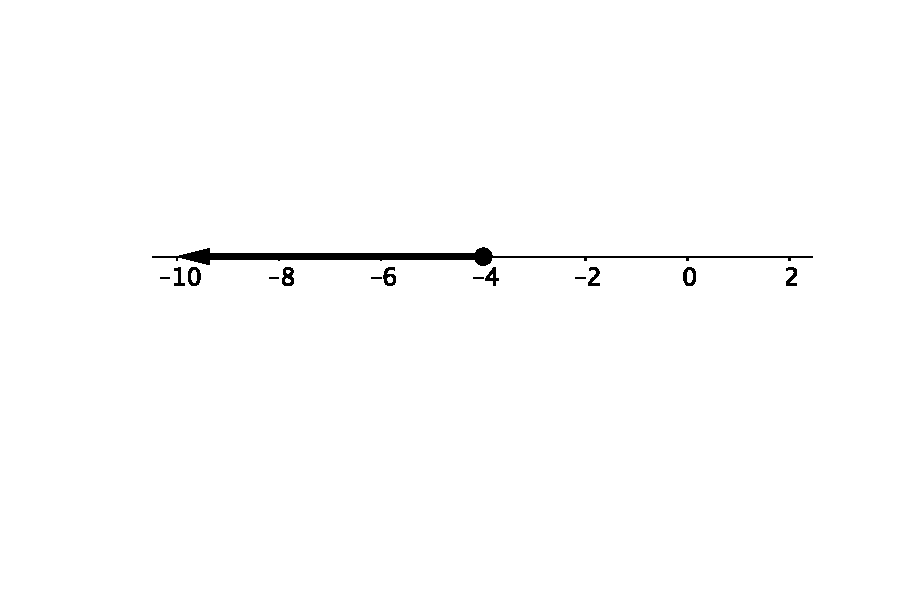
\includegraphics{fig095-07-5-c-answer}\end{center}\end{onlysolution}
}
{
	\begin{tabular}{l r}
	$\dfrac{10}{1}\left(\dfrac{4}{5}x+2\right) \leq \dfrac{10}{1}\left(\dfrac{3}{10}x\right)$ & 1 pt to here \\
	$8x+20\leq 3x$ & 2 pts to here \\
	$x\leq -4$ OR $-4\geq x$ & 3 pts to here \\
	 & add 2 pts for correct number line.
	\end{tabular}
}

\newproblem{07.5d}
{
	Solve and graph on the number line. $$\frac{1}{3}x-1 \geq \frac{5}{6}x$$\begin{onlyproblem}\begin{center}
\includegraphics{numberLineNoNumbersNoTicks}\end{center}\end{onlyproblem} \begin{onlysolution}\begin{center}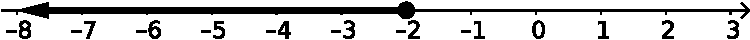
\includegraphics{fig095-07-5-d-answer}\end{center}\end{onlysolution}
}
{
	\begin{tabular}{l r}
	$\dfrac{6}{1}\left(\dfrac{1}{3}x-1\right)\geq \dfrac{6}{1}\left(\dfrac{5}{6}x\right)$ & 1 pt to here \\
	$2x-6\geq 5x$ & 2 pts to here \\
	$x\leq -2$ OR $-2\geq x$ & 3 pts to here \\
	 & add 2 pts for correct number line.
	\end{tabular}
}
